%%%%%%%%%%%%%%%%%%%%%%%%%%%%%%%%%%%%%%%%%%%%%%%%%%%%%%%%%%%%%%%%%%%%%%%%%%%%%%%
%% LaTeX-Vorlage für Abschlussarbeiten                                       %%
%% (TH Köln -Campus Gummersbach, Fak. 10)                                    %%
%%                                                                           %%
%% Gemäß dem Merkblatt zur Anfertigung von Projekt-, Bachelor-, Master- und  %%
%% Diplomarbeiten der Fakultät 10 von Frau Prof. Dr. Halfmann &              %%
%% Herr Prof. Dr. Rühmann (Version vom 27.01.2008)                           %%
%%                                                                           %%                                                                            
%% Bitte sprechen Sie unbedingt mit Ihrer Betreuerin bzw. Ihrem Betreuer     %%
%% bezüglich der Ausgestaltung Ihrer Arbeit!                                 %%
%%                                                                           %%
%%                                                                           %%
%% MERKKASTEN IN DIESER VORLAGE:                                             %%
%% In dieser Vorlage finden Sie Merkkasten, die Ihnen Informationen          %%
%% zu bestimmten, formalen Aspekten geben. Sprechen Sie immer auch mit       %% 
%% Ihrer Betreuerin bzw. Ihrem Betreuer dazu an.                             %%                       
%% Für die eigene Verwendung der Vorlage entfernen oder kommentieren Sie die %%
%% Merkkasten. Die betreffenden Bereiche für die Merkkasten in der Vorlage   %%
%% sind wie folgt kommentiert: <MERKKASTEN> ... </MERKKASTEN>.               %%                            %%                                                                           %%
%%                                                                           %%
%% LIZENZ:                                                                   %%
%% Diese Vorlage darf nicht kommerziell verbreitet                           %%
%% werden. Eine nicht-kommerzielle Weitergabe ist                            %% 
%% gestattet.                                                                %%
%%                                                                           %%
%% Von Ludger Schönfeld, M. Sc.,
%% 2014-2017                            %%
%%%%%%%%%%%%%%%%%%%%%%%%%%%%%%%%%%%%%%%%%%%%%%%%%%%%%%%%%%%%%%%%%%%%%%%%%%%%%%%

%%%%%%%%%%%%%%%%%%%%%%%%%%%%%%%%%%%%%%%%%%%%%
%% HEADER                                  %%
%%%%%%%%%%%%%%%%%%%%%%%%%%%%%%%%%%%%%%%%%%%%%
\documentclass[a4paper,12pt,oneside]{article}
% Optionen:
% - a4paper => DIN A4-Format
% - 12pt    => Schriftgröße (weitere  
%              grundlegende Fontgrößen: 10pt, 11pt)
% - oneside => Einseitiger Druck

%% Verwendete Pakete:
\usepackage[ngerman]{babel} % für die deutsche Sprache
\usepackage{caption} % Für schönere Bildunterschriften
\usepackage[T1]{fontenc} % Schriftkodierung (Für Sonderzeichen u.a.)
\usepackage[utf8]{inputenc} % Für die direkte Eingabe von Umlauten im Editor u.a.
\usepackage{fancyhdr} % Für Kopf- und Fußzeilen
\usepackage{lscape} % Für Querformat
% !TeX spellcheck = de_DE
%% Schriften (Beispiele)
%% Weitere LaTeX-Schriften im "LaTeX Font Catalogue"
%% unter: http://www.tug.dk/FontCatalogue/.
%% ACHTUNG: Ggf. müssen Schriften noch installiert 
%% werden!

% Serifen-Schriften:
\usepackage{lmodern} % Schriftart "Latin Modern"
%\usepackage{garamond} % Schriftart "Garamond"

%Sans Serif-Schriften:
%\usepackage[scaled]{uarial}
%\usepackage[scaled]{helvet}
%%--------------
\usepackage[normalem]{ulem} % Für das Unterstreichen von Text z.B. mit \uline{}
\usepackage[left=3cm,right=2cm,top=1.5cm,bottom=1cm,
textheight=245mm,textwidth=160mm,includeheadfoot,headsep=1cm,
footskip=1cm,headheight=14.599pt]{geometry} % Einrichtung der Seite 

\usepackage{graphicx} % Zum Laden von Graphiken
% INFO: Graphiken einbinden
%
% \includegraphics[scale=1.00]{dateiname}
%
% => Ausgabeformat: PDF-Dokument:
%    Es können die folgenden (Graphik-)formate eingebunden
%    werden: .jpg, .png, .pdf, .mps
% 
% => Ausgabeformat: DVI/PS:
%    Folgende (Graphik-)formate werden unterstützt:
%    .eps, .ps, .bmp, .pict, .pntg
\usepackage{epstopdf}

% Pakete für Tabellen
\usepackage{tabularx} % Einfache Tabellen
\usepackage{longtable} % Tabellen als Gleitobjekte (für die Aufteilung bei langen 
 %Tabellen über mehrere Seiten)
\usepackage{multirow} % Für das Verbinden von Zeilen innerhalb einer Tabelle mit
 % \multirow{anzahl}{*}{Text}

% (Zusatz-)Pakete für Formeln
\usepackage{amsmath}
\usepackage{amsthm}
\usepackage{amsfonts}

\usepackage{setspace} % Paket zum Setzen des Zeilenabstandes
% INFO: Zeilenabstand setzen:
%
% Befehle:
% - \singlespacing  => 1-zeilig (Standard)
% - \onehalfspacing => 1,5-zeilig
% - \doublespacing  => 2-zeilig 
\onehalfspacing % Zeilenabstand auf 1,5-zeilig setzen

% Farbboxen (für die Merkkästen in dieser Vorlage):
\usepackage{tcolorbox}
\tcbset{colback=white,colframe=orange,
        fonttitle=\bfseries}

\usepackage[colorlinks,pdfpagelabels,pdfstartview=FitH,
bookmarksopen=true,bookmarksnumbered=true,linkcolor=black,
plainpages=false,hypertexnames=false,citecolor=black]{hyperref} % Für Verlinkungen
% INFO: Verlinkungen mit dem hyperref-Paket:
%
% Die Angabe von URLs mit dem Befehl \url{} erlaubt einen
% gesonderten Umgang mit Weblinks. Denn die Links werden verlinkt.
% Auch erfolgt automatisch am Zeilenende ein Umbruch des Links.
% Es ist auch nicht erforderlich, Sonderzeichen in der URL manuell zu 
% entschärfen.
%
% TIPP: Sollte ein Umbuch bei einem Link nicht automatisch erfolgen, so kann
% das daran liegen, dass ein/mehrere Zeichen zusätzlich angegeben werden müssen,
% an dem der Link umbrochen werden kann.
% Dies kann mit folgendem Befehl erfolgen (Beispiel):
% \renewcommand*\UrlBreaks{\do-\do_}

% Das Paket "biblatex" für autom. 
% Literaturverzeichnisse:
%\usepackage{csquotes} % Für sprachangepasste Anführungszeichen
%\usepackage[backend=bibtex,style=alphabetic]  
%           {biblatex}
%\addbibresource{bib/literatur.bib}           

%%%%%%%%%%%%%%%%%%%%%%%%%%%%%%%%%%%%%%%%%%%%%
%% DOKUMENT                                %%
%%%%%%%%%%%%%%%%%%%%%%%%%%%%%%%%%%%%%%%%%%%%%
\begin{document}
  % Unbeschriftetes Vorblatt (Leere Seite)
  \pagestyle{empty} % Seite ohne Kopf- und Fußzeilen
 % \section*{}  
           % Ausgelagerte LaTeX-Datei (hier: leereSeite.tex) einbinden
  
  % Deckblatt
  \pagestyle{empty}
  \begin{titlepage}
    
\includegraphics[scale=1.00]{Sources/logo_TH-Koeln_CMYK_22pt}\\
    \begin{center}
      \Large
      Technische Hochschule Köln\\
      Fakultät für Informations-, Medien- und Elektrotechnik (F07)\\
      \hrule\par\rule{0pt}{2cm} % Horizontale Trennlinie  mit 2 cm Abtand nach unten erzeugen
      \LARGE
      \textsc{B A C H E L O R A R B E I T}\\
      \vspace{1cm} % Vertikaler Abstand von 1cm erzeugen
      \huge
      Entwicklung eines Tools zum Vergleich textbasierter Dateien mit graphischer Anzeige der Unterschiede\\
      \vspace{1.5cm}
      \large
      Vorgelegt an der TH Köln\\
      Campus Deutz\\
      im Studiengang\\
      Technische Informatik B.Sc.\\ 
      \vspace{1.0cm}
      ausgearbeitet von:\\
      \textsc{Allen Kletinitch}\\
      (Matrikelnummer: 11124870)\\
      \vspace{1.5cm}
      \begin{tabular}{ll} % Einfache Tabelle ohne Rahmen, mit 2 Spalten erzeugen
          \textbf{Erster Prüfer:} & Prof. Dr. Rainer Bartz \\
          \textbf{Zweiter Prüfer:} & Prof. Dr. René Wörzberger \\
      \end{tabular}
      \vspace{1.0cm}
      \newline Juli 2021\\
    \end{center}    
  \end{titlepage}
  
  \newpage
  
  % Abstract (ACHTUNG: Abweichung zur Reihenfolge im Merkblatt!)

  % !TeX root = ../BA_LateXVorlage_v3-2.tex
\begin{center}
\renewcommand{\abstractname}{Titel}
\begin{abstract}
\noindent Entwicklung einer Software zum Vergleich textbasierter Dateien mit graphischer Anzeige der Unterschiede und besonderem Fokus auf XML und JSON
\end{abstract}

\renewcommand{\abstractname}{Zusammenfassung}
\begin{abstract}\label{abstract} 
\noindent
Wachsende Datenmengen sind ein stetiger Trend in der Informatik. Häufig können Anwendungsfälle gefunden werden bei denen es interessant ist die Unterschiede zwischen diesen Daten, bspw. bei der Versionierung, zu untersuchen. Im Rahmen dieser Bachelorarbeit wird eine Software erstellt, die beliebig viele textbasierte Dateien miteinander vergleicht, ihre Ähnlichkeit quantifiziert und die Möglichkeit bietet, Unterschiede für bis zu drei Dateien graphisch im Detail nachzuvollziehen. 
Weiterhin werden besondere Operationen für die gängigen Dateiformate XML und JSON implementiert um deren Inhalte sinnvoll vergleichbar zu machen. Zusätzlich werden für diese Dateiformate spezialisierte Vergleichsalgorithmen auf Basis ihrer Dokumentbäume entworfen und implementiert.

\vspace{1.0cm}
\noindent \textbf{Stichwörter: }Textvergleich, Diff, XML, JSON
 
\end{abstract}







\vspace{1.5cm}

\renewcommand{\abstractname}{Title}
\begin{abstract}
\noindent Development of a software to compare text-based files with graphical display of differences and special focus on XML and JSON
\end{abstract}

\renewcommand{\abstractname}{Abstract}
\begin{abstract}
\noindent
Growing amounts of data are a constant trend in computer science. Frequently, use cases can be found where it is interesting to look at the differences between parts of this data, for example in the case of versioning. In the context of this bachelor thesis a software is created, which compares arbitrarily many text-based files with each other, quantifies their similarity and offers the possibility to trace differences graphically in detail for up to three files. 
Furthermore, special operations for the common file formats XML and JSON are implemented to make their contents meaningfully comparable. Additionally, specialized comparison algorithms are designed and implemented for these file formats based on their document trees.


\vspace{1.0cm}
\noindent \textbf{Keywords: }text comparison, diff, XML, JSON
\end{abstract}



\end{center}

  \newpage
  
  % Inhaltsverzeichnis
  \tableofcontents
  
  \newpage
  \pagestyle{fancy} % Kopf- und Fußzeilen aktivieren (=> Paket "fancyhdr")
 
  % Abbildungsverzeichnis  
  % INFO: Abbildung einbinden (Beispiel):
  %  \begin{figure}[h!]
  %    \centering
  %    \includegraphics[scale=1.00]{Pfad zum Bild}\\
  %    \caption{Bildunterschrift} 
  %    \label{Marke zum Referenzieren auf die Abbildung}
  %  \end{figure}
  \section*{Abbildungsverzeichnis}
  \addcontentsline{toc}{section}{Abbildungsverzeichnis} % Manuellen Eintrag im Inhaltsverzeichnis erzeugen
  \renewcommand{\listfigurename}{} % Name des Abbildungsverzeichnisses ändern
  \thispagestyle{empty}
  \listoffigures
  
  \newpage
  
  % Tabellenverzeichnis
  %\addcontentsline{toc}{section}{Tabellenverzeichnis}
  %\listoftables
  
  %\newpage
  
  % Hauptteil des Dokuments
  % TIPP: Jedes Kapitel oder jeder Abschnitt in eine eigene
  % LaTeX-Datei (.tex) auslagern.
  % Einbinden der ausgelagerten Dateien in diese Hauptdatei, erfolgt 
  % mittels folgendem Befehl (Beispiel):
  % beispiel.tex => \input{beispiel}
  \newpage
  % !TeX root = ../BA_LateXVorlage.tex
\section{Einleitung} 
Bereits seit der Industrialisierung sind Menschen bemüht ihre Aufgaben zu automatisieren. Diese Entwicklung hat auch in den letzten Jahren nicht stagniert. Besonders in der Informatik finden sich viele Themengebiete, die versuchen dem Menschen Arbeit durch Automatisierung abzunehmen. Sie existieren bspw. im Feld des Machine Learnings beim autonomen Fahren. Durch den Einsatz komplexer Algorithmen soll es der Person hinter dem Lenkrad ermöglicht werden ohne eigenen Einsatz an ihr Ziel zu kommen.

Auch im Cloud Computing findet Automatisierung Platz. Dort wird die Skalierbarkeit von cloudbasierten Software-Systemen immer seltener von Mitarbeitenden manuell eingestellt, um die Verfügbarkeit der Systeme zu versichern. Für solche Zwecke werden Orchestrierungstools wie Kubernetes eingesetzt, die die Systeme anhand von Konfigurationsdateien automatisch auf die verfügbare Hardware-Infrastruktur verteilen. Allerdings sind diese Dateien selbst nicht automatisch generiert, sondern müssen manuell erstellt werden.

Ein Beispiel für automatisch generierte Dateien findet sich ebenfalls beim Machine Learning im Bereich der Objekterkennung. Für ein System, welches Objekte auf Bildern erkennen soll, werden große Mengen an Bilddateien für das Training des Systems bereitgestellt. Beim Testen wertet das System anschließend Bilder aus auf denen es nicht trainiert wurde, und kann automatisch für jedes dieser Bilder eine Datei erstellen, die unter anderem die Klassifikation gefundener Objekte und deren Lokalisierung mit Objektmasken oder Objektbegrenzungen dokumentiert \autocite[]{coco-article}\autocite[]{cocoOutput}. 

\subsection{Motivation}
Gerade bei dem Beispiel der Objekterkennung können riesige Dateimengen entstehen. Dabei ist es oft interessant zu betrachten, wie sich das System im Laufe der Entwicklung verändert und ob sich die Genauigkeit der Erkennung verbessert. Es kann nämlich sein, dass das System in früheren Durchläufen ähnliche, aber falsche Objekte erkennt und sich über den Trainingszeitraum dahingehend verbessert, dass die Objekte nun richtig erkannt werden.

Um diese Verbesserung nachzuvollziehen, müssten zunächst die Dateien gesucht werden, die mit dem gleichen Bild korrespondieren. Diese haben zum Beispiel einen ähnlichen Namen und liegen dann nach Durchlauf getrennt in verschiedenen Verzeichnissen. Nachdem diese Dateien gefunden wurden, müssen sie in einem Texteditor geöffnet und nach Unterschieden durchsucht werden. Für wenige Dateien ist das zwar möglich, aber selbst dann kann es schon Zeitaufwändig werden.

Diese Arbeit fokussiert sich deshalb auf die Weiterentwicklung einer Software, die dazu dient beliebig viele Dateien aus dem Dateibaum einzulesen, ihre Ähnlichkeit zu quantifizieren und mögliche Unterschiede graphisch darzustellen.

\subsection{Ausgangssituation}
Im Vorfeld dieser Arbeit ist bereits im Rahmen eines Projekts im Studiengang Technische Informatik an der Technischen Hochschule Köln eine erste Version dieser Software entstanden. Es handelt sich dabei um die Software MultiTextCompare; eine Desktop-Anwendung für Windows Betriebssysteme, die bereits grundlegende Implementierungen für einige der notwendigen Funktionen bereitstellt. Es ist möglich, Dateien des selben Dateityps nach Name oder Namensmuster, wie etwa im Windows-Explorer, automatisch einzulesen. Dafür muss lediglich ein Wurzelverzeichnis angegeben werden, unter dem alle Unterverzeichnisse nach passenden Dateien durchsucht werden. Im nächsten Schritt hat der Benutzer die Wahl, ob die ausgewählten Dateien nach bestimmten Parametern normiert werden sollen oder nicht. Aktuell werden die Dateiendungen txt, xml und json unterstützt und für jeden dieser Dateitypen stehen andere Parameteroptionen zur Verfügung. Für reguläre Textdokumente können Operationen wie das Entfernen von Leerzeichen, Leerzeilen, Satzzeichen oder Groß- und Kleinschreibung durchgeführt werden. Für die Formate \acrshort{xml} und \acrshort{json} gibt es zusätzliche Operationen auf Basis von Parsern, die u.\,a. die Sortierung der Dokumentbäume ermöglichen. 

Nach dieser Normierung findet der eigentliche Vergleich statt. Dem Benutzer werden zwei unterschiedliche Vergleichsmodi angeboten. Zum einen können die Dateien Wort für Wort verglichen werden, zum anderen können auch die gesamten Zeichenmengen auf Ähnlichkeit überprüft werden. Auf die genaue Funktionsweise der beidem Modi wird später in der Arbeit noch im Detail eingegangen. Nachdem alle Dateien miteinander verglichen wurden, wird eine kolorierte Matrix mit allen Vergleichsergebnissen angezeigt (siehe Abb. \ref{fig:matrix_v1}). Ähnliche Dateien werden grün dargestellt, stark verschiedene rot. Bei der Ähnlichkeit handelt es sich des weiteren um einen prozentualen Wert, d.\,h. dass identische Dateien eine Ähnlichkeit von 1 haben, und der Minimalwert 0 ist. 

\begin{figure}[!htb]
    \centering
    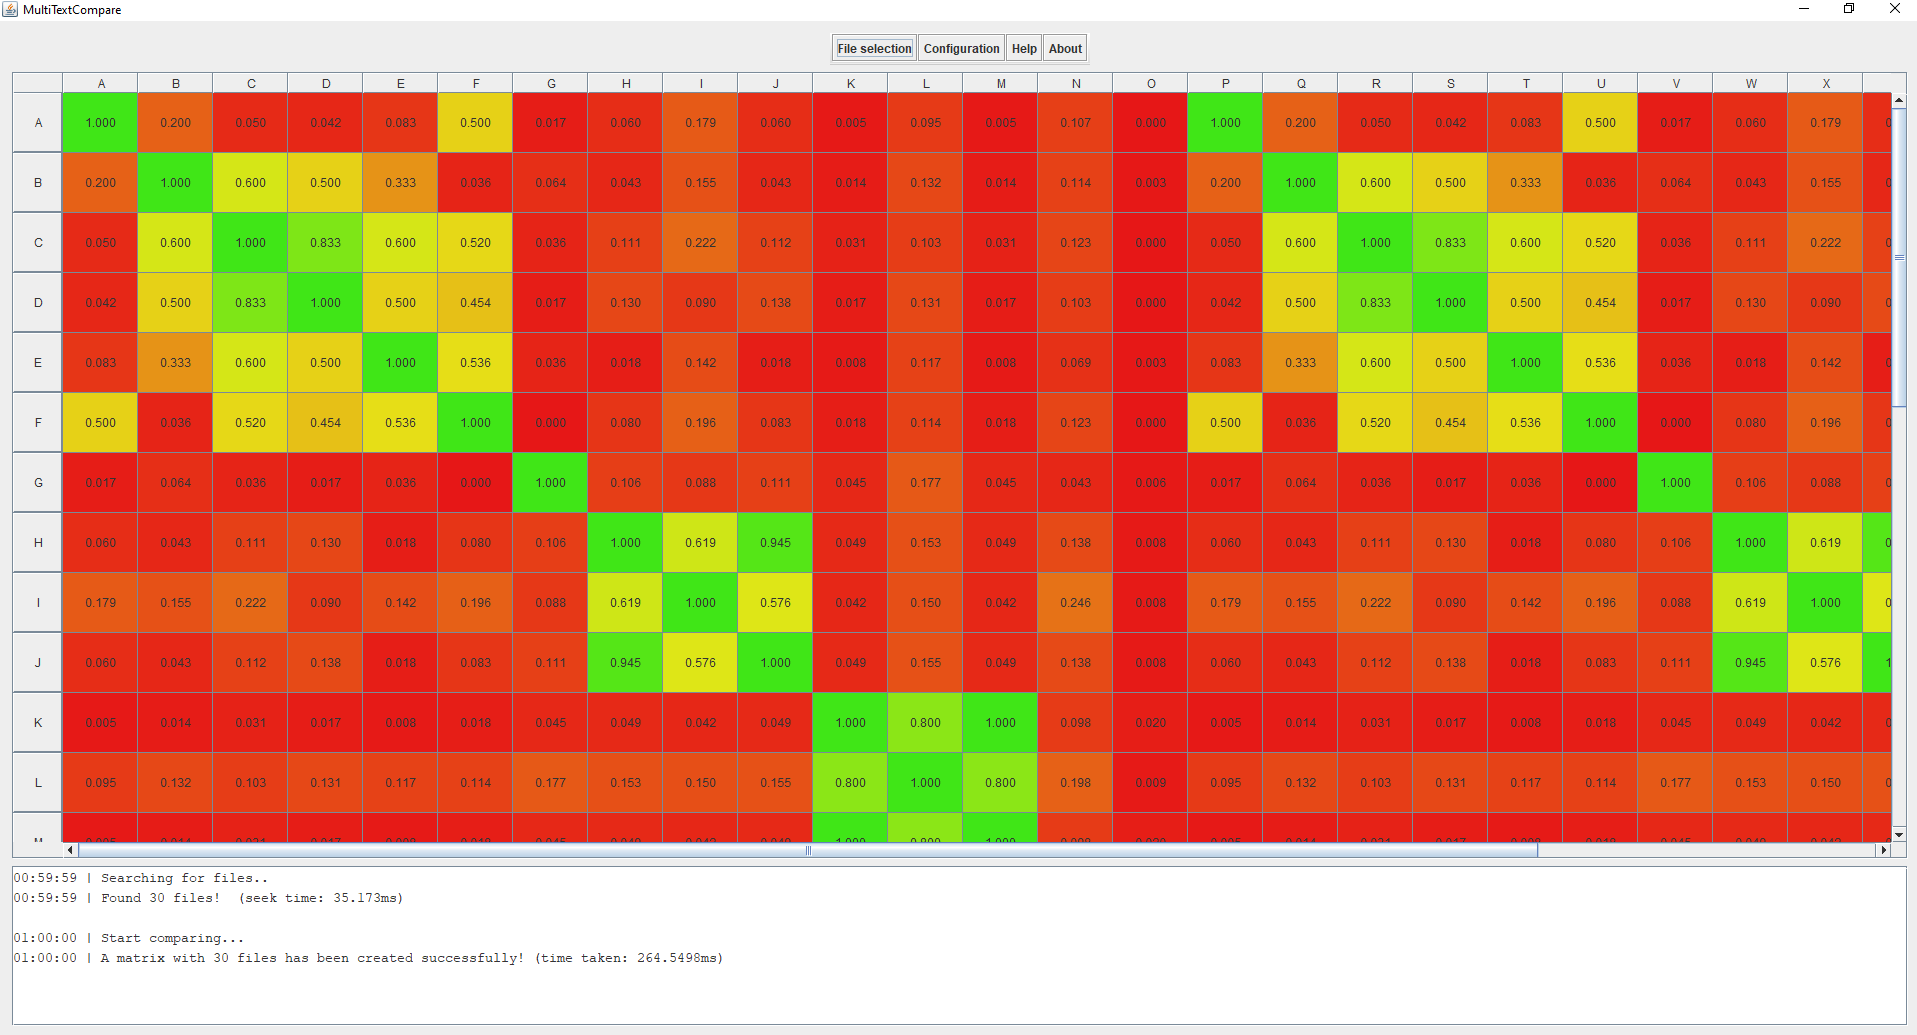
\includegraphics[scale=0.25]{images/matrix V1.png}
    \caption{Ähnlichkeitsmatrix in Version 1.0}
    \label{fig:matrix_v1}
\end{figure}

Zuletzt kann der Benutzer dann auf die einzelnen Zellen der Matrix klicken, um sich die Unterschiede für zwei oder drei Dateien gleichzeitig farbig markieren zu lassen. Dieser Stand der Software wird fortan als Version 1.0 referenziert.

\subsection{Zielsetzung}\label{zielsetzung}
Ziel dieser Arbeit ist es, die Software MultiTextCompare an den nötigen Stellen zu verbessern. Dazu zählen hauptsächlich die Benutzerfreundlichkeit, Laufzeit und die Genauigkeit der Vergleichsalgorithmen.

Dabei gliedert sich die Arbeit in 6 Kapitel: Die theoretischen Grundlagen, die Konzeption der Software, die Implementierung der Verbesserungen, deren Verifikation sowie die Zusammenfassung mit Ausblick.

Die theoretischen Grundlagen sollen zunächst in das Thema des Textvergleichs einleiten. Dafür wird der Begriff der Ähnlichkeit von Zeichenketten diskutiert und anhand von zwei verschiedenen Textvergleichsalgorithmen dargestellt. Darauf folgt eine Übersicht zu den Dateiformaten \acrshort{xml} und \acrshort{json} und eine Vorstellung der speziellen Aspekte in der Programmierung der Software. Dort geht es dann beispielsweise um die Funktionsweise des UI-Toolkits Java Swing und die Implementierung von Nebenläufigkeit in Java.

Das Kapitel zur Konzeption zieht anschließend einen Vergleich zu bereits bestehender Software, deren Vorteilen und ihren Limitationen. Danach werden kurz die besonderen Aspekte für die Entwicklung dargestellt. Darunter liegen bspw. die zu verwendenden Bibliotheken und Tools und die Limitationen der Systeme auf denen die Software lauffähig sein soll. Zuletzt gibt es einen kurzen Überblick über die bestehende Architektur der Software und der Codebase.

In Kapitel 4 geht es hauptsächlich um die durchzuführenden Aufgaben dieser Arbeit. Es wird also konkret die Vorgehensweise bei der Entwicklung erklärt. Dabei soll auch gezeigt werden, durch welche Probleme eine Änderung der Funktionalität notwendig ist, und wie diese Probleme gelöst werden können. Für die Dateiformate \acrshort{xml} und \acrshort{json} sollen zudem eigene Vergleichsalgorithmen entworfen werden, die nun nicht mehr auf reiner Textbasis arbeiten, sondern sich explizit mit den Baumstrukturen der Dokumente auseinandersetzen, um dort einen spezialisierten Vergleich durchführen zu können.

Das fünfte Kapitel beschäftigt sich dann ausführlich mit der Verifikation der in Kapitel 4 durchgeführten Laufzeitoptimierungen und den neuen Vergleichsalgorithmen. Dabei werden die Testsysteme vorgestellt, die Methodik erklärt und die Ergebnisse kritisch evaluiert.

Im letzten Kapitel befindet sich abschließend eine Zusammenfassung der durchgeführten Entwicklungen und der gewonnenen Erkentnisse und ein Ausblick, wie die Software in Zukunft noch weiter verbessert werden könnte.
  % INFO: Querverweise auf Gliederungselemente, Abbildungen 
  %       & Tabellen setzen:
  %
  % Voraussetzung: Gesetzte Referenzmarke mit dem Befehl: \label{marke}
  % 
  % Referenzierung erfolgt dann mittels dem Befehl:
  % \ref{marke}
  
  %\section{Einleitung}\label{kap_einleitung}  
   %\input{} 
   TEXT FOLGT...
   
  \newpage  
  \section{Grundlagen}\label{kap_grundlagen}  
    TEXT FOLGT...
   
    \subsection{Unterabschnitt von Grundlagen}\label{subsec_UabsGrundl}
     %\input{}
     TEXT FOLGT... 
  
  
  \newpage 
  \section{Zusammenfassung und Ausblick}\label{kap_zusammfAusbl}  
   %\input{}
   TEXT FOLGT...
  % Literaturverzeichnis
   % INFO: Referenzieren auf das Literaturverzeichnis:
   %
   % Befehl: \cite{refmarke}
   % 
   % "refmarke" ist die Angabe in den geschweiften Klammern bei 
   % \bibitem[]{refmarke}. 
   \newpage
    \thispagestyle{empty}
   \section{Quellenverzeichnis}
     \subsection{Literatur}
     \renewcommand{\refname}{} % Literaturverzeichnis ohne Bezeichnung
     % Variante 1: einfaches, manuelles 
     % Literaturverzeichnis
     \begin{thebibliography}{SW11} % 2. {...} => Hier die größte /breiteste Nummer (z.B. 99) oder Kurzbeleg angeben.
       \bibitem[SW11]{SW11} Stickel-Wolf, Christine; Wolf, Joachim (2011): Wissenschaftliches Lernen und Lerntechniken. Erfolgreich studieren–-gewusst wie!. Wiesbaden: Gabler. 
     \end{thebibliography} 
          
     \subsection{Internetquellen}
     \begin{thebibliography}{HR08} % 2. {...} => Hier die größte/breiteste Nummer (z.B. 99) oder Kurzbeleg angeben.
       \bibitem[BBoJ]{BBoJ}Bertelsmeier, Birgit (o. J.): Tipps zum Schrei\-b\-en ei\-n\-er Ab\-sch\-luss\-ar\-beit. Fach\-hoch\-schu\-le Köln-Campus Gummersbach, Institut für Informatik. \url{http://lwibs01.gm.fh-koeln.de/blogs/bertelsmeier/files/2008/05/abschlussarbeitsbetreuung.pdf} (29.10.2013).
        \bibitem[HR08]{HR08} Halfmann, Marion; Rühmann, Hans (2008): Merkblatt zur Anfertigung von Projekt-, Bachelor-, Master- und Diplomarbeiten der Fakultät 10. Fachhochschule Köln-Campus Gummersbach.\url{http://www.f10.fh-koeln.de/imperia/md/content/pdfs/studium/tipps/anleitungda270108.pdf} (29.10.2013).
     \end{thebibliography} 
  
  % INFO: Biblatex -Ausgabe des  
  % Literaturverzeichnisses (Beispiele):   
  % - \printbibliography => Ausgabe ALLER 
  %   Einträge
  % - \printbibliography[nottype=online]
  %   => Ausgabe der Einträge, bis auf die
  %      "Online"-Einträge
  % - \printbibliography[type=online]     
  %   => Ausgabe nur der "Online"-Einträge  
   %\printbibliography

  % Anhang
  \newpage
  \setcounter{section}{0} % Nummerierung der Gliederungsebene "section" auf 0 setzen
  \renewcommand*\thesection{\Alph{section}} % Nummerierungsart für die Gliederungsebene "section" 
  % auf Großbuchstaben setzen
  \section{Anhang}\label{anhang}
    \subsection{Unterabschnitt von Anhang}\label{subsec_UabsAnhang}
    TEXT FOLGT...
  
  \newpage
  
 % Erklärung über die selbständige Abfassung der Arbeit  
 \pagestyle{empty}
 \section*{Erklärung über die selbständige\\Abfassung der Arbeit} % \section*{...}: das *-Symbol erlaubt, dass dieser
 % Gliederungspunkt nicht ins Inhaltsverzeichnis aufgenommen wird
 \addcontentsline{toc}{section}{Erklärung über die selbständige Abfassung der Arbeit}
 Ich erkläre an Eides statt, dass ich die vorgelegte Abschlussarbeit selbständig und
 ohne fremde Hilfe verfasst, andere als die angegebenen Quellen und Hilfsmittel
 nicht benutzt und die den benutzten Quellen wörtlich oder inhaltlich entnommenen
 Stellen als solche kenntlich gemacht habe.\\\\
\begin{tabular}{cp{7cm}}
    & \\ 
    & \\ \hline
  \small (Ort, Datum, Unterschrift) & \normalsize \\
  \end{tabular} 
   
\newpage
% Unbeschriftetes Abschlussblatt (Leere Seite)
\thispagestyle{empty}
\section*{}  
          
    
\end{document}

